
\chapter{Sidereal Systems}

\lettrine[lines=4]{\goudy T}{his} position of our solar system, and the form of the whole discoidal stratum, have been inferred from sidereal scales, that is to say, from that method of counting the stars to which I have already alluded, and which is based upon the equidistant subdivision of the telescopic field of view. The relative depth of the stratum in all directions is measured by the greater or smaller number of stars appearing in each division. These divisions give the length of the ray of vision in the same manner as we measure the depth to which the plummet has been thrown, before it reaches the bottom, although in the case of a starry stratum there can not, correctly speaking, be any idea of depth, but merely of outer limits. In the direction of the longer axis, where the stars lie behind one another, the more remote ones appear closely crowded together, united, as it were, by a milky white radiance or luminous vapor, and are perspectively grouped, encircling, as in a zone, the visible vault of heaven. This narrow and branched girdle, studded with radiant light, and here and there interrupted by dark spots, deviates only by a few degrees from forming a perfect large circle round the concave sphere of heaven, owing to our being near the center of the large starry cluster, and almost on the plane of the Milky Way. If our planetary system were far outside this cluster, the Milky Way would appear to telescopic vision as a ring, and at a still greater distance as a resolvable discoidal nebula.
\clearpage
\begin{figure}[h]
    \centering
    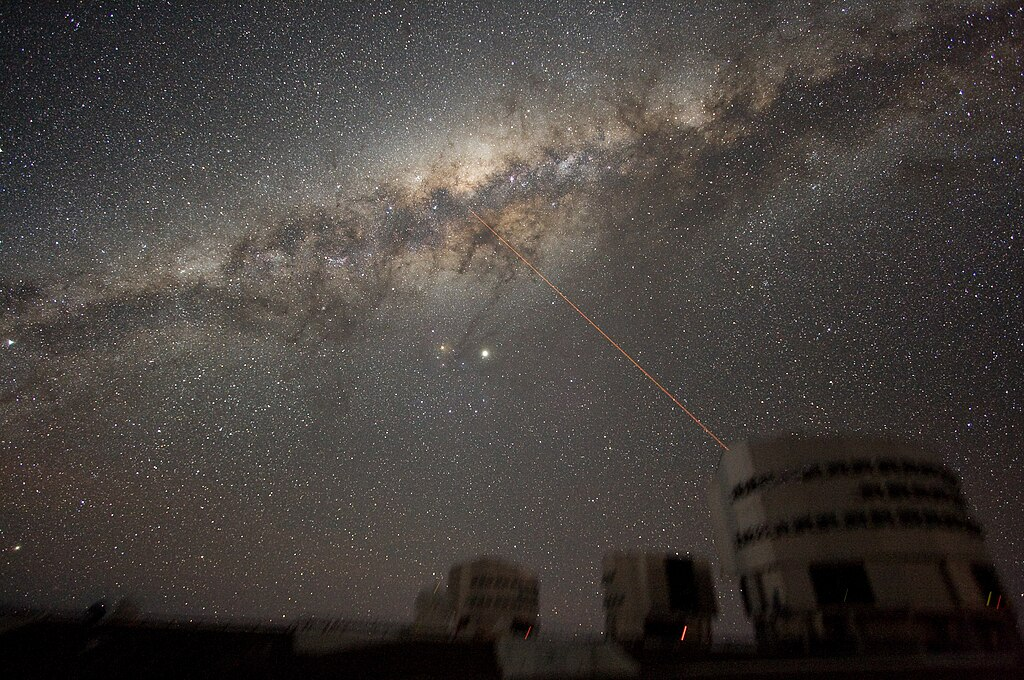
\includegraphics[width=.9\textwidth]{../../pictures/ESO-VLT-Laser-phot-33a-07.jpg}
    \caption{The Galactic Center as seen from Earth's night sky (featuring the telescope's laser guide star). Listed below is Galactic Center's information. Author: \href{https://en.wikipedia.org/wiki/File:ESO-VLT-Laser-phot-33a-07.jpg}{ESO/Y. Beletsky}. License: \href{https://creativecommons.org/licenses/by/4.0}{CC BY 4.0}.}
    \label{fig:eso-vlt-laser}
\end{figure}

Among the many self-luminous moving suns, erroneously called fixed stars, which constitute our cosmical island, our own sun is the only one known by direct observation to be a central body in its relations to spherical agglomerations of matter directly depending upon and revolving round it, either in the form of planets, comets, or aërolite asteroids. As far as we have hitherto been able to investigate multiple stars (double stars or suns), these bodies are not subject, with respect to relative motion and illumination, to the same planetary dependence that characterizes our own solar system. Two or more self-luminous bodies, whose planets and moon, if such exist, have hitherto escaped our telescopic powers of vision, certainly revolve around one common center of gravity; but this is in a portion of space which is probably occupied merely by unagglomerated matter or cosmical vapor, while in our system the center of gravity is often comprised within the innermost limits of a visible central body. If, therefore, we regard the Sun and the Earth, or the Earth and the Moon, as double stars, and the whole of our planetary solar system as a multiple cluster of stars, the analogy thus suggested must be limited to the universality of the laws of attraction in different systems, being alike applicable to the independent processes of light and to the method of illumination.

For the generalization of cosmical views, corresponding with the plan we have proposed to follow in giving a delineation of nature or of the universe, the solar system to which the Earth belongs may be considered in a twofold relation  first, with respect to the different classes of individually agglomerated matter, and the relative size, conformation, density, and distance of the heavenly bodies of this system; and, secondly, with reference to other portions of our starry cluster, and of the changes of position of its central body, the Sun.